\documentclass[tikz,border=6pt]{standalone}
\usepackage{amsmath,amssymb}
\usetikzlibrary{arrows.meta,calc}
\definecolor{ink}{HTML}{102B42}
\definecolor{bluefill}{HTML}{BBD5F1}
\definecolor{greenfill}{HTML}{C4E3BA}
\definecolor{yellowfill}{HTML}{D9E9F8}
\definecolor{pinkfill}{HTML}{E7A8BC}
\begin{document}
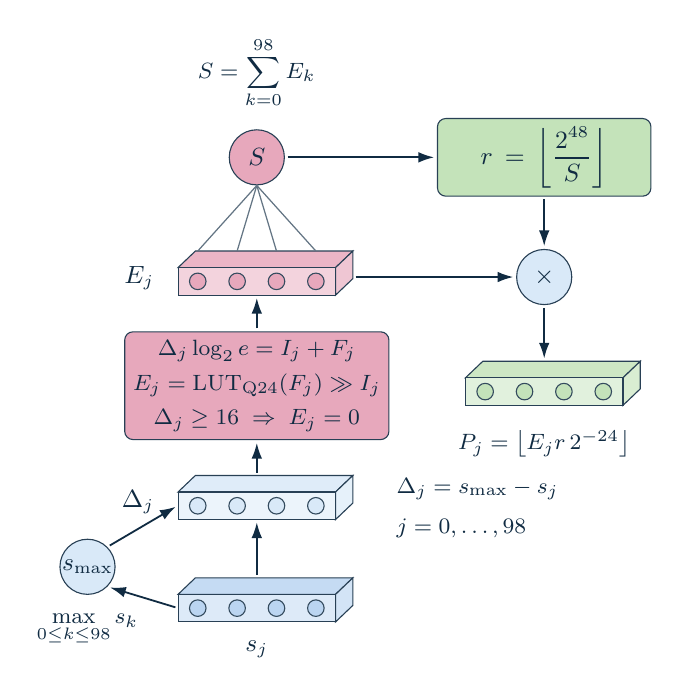
\begin{tikzpicture}[font=\small,text=ink,>=Latex,
 arr/.style={-{Latex[length=2mm,width=1.35mm]},draw=ink,line width=.65pt,shorten <=1pt,shorten >=1pt},
 link/.style={draw=ink!65,line width=.45pt},
 box/.style={draw=ink!90,rounded corners=3pt,align=center,inner sep=3pt,fill=greenfill},
 dot/.style={circle,draw=ink!90,fill=yellowfill,minimum size=7mm,inner sep=0pt}]
% A row vector is shown as a shallow three-dimensional block.
\newcommand{\vectorblock}[4]{%
 \begin{scope}[shift={(#1,#2)}]
 \filldraw[fill=#3!85,draw=ink!90] (0,.35)--(.22,.56)--(2.22,.56)--(2,.35)--cycle;
 \filldraw[fill=#3!65,draw=ink!90] (2,0)--(2.22,.21)--(2.22,.56)--(2,.35)--cycle;
 \filldraw[fill=#3!50,draw=ink!90] (0,0) rectangle (2,.35);
 \foreach \x in {.25,.75,1.25,1.75}{\filldraw[fill=#3,draw=ink!85] (\x,.175) circle (.105);}
 \node[anchor=east,align=right] at (-.18,.22) {#4};
 \end{scope}}

\vectorblock{0}{0}{bluefill}{}
\node[anchor=north] at (1,-.12) {$s_j$};
\vectorblock{0}{1.3}{yellowfill}{}
\node[anchor=east] at (-.18,1.52) {$\Delta_j$};
\node[dot,fill=yellowfill] (max) at (-1.15,.7) {$s_{\max}$};
\node[anchor=north,font=\footnotesize] at (-1.15,.22) {$\displaystyle\max_{0\le k\le98}s_k$};
\draw[arr] (0,.175)--(max.south east);
\draw[arr] (max.north east)--(0,1.48);
\draw[arr] (1,.56)--(1,1.3);
\node[box,fill=pinkfill,font=\footnotesize] (exp) at (1,3.0) {$\Delta_j\log_2 e=I_j+F_j$\\[3pt]
$E_j=\mathrm{LUT}_{\mathrm{Q24}}(F_j)\gg I_j$\\[3pt]
$\Delta_j\ge16\;\Rightarrow\;E_j=0$};
\draw[arr] (1,1.86)--(exp.south);
\vectorblock{0}{4.15}{pinkfill}{$E_j$}
\draw[arr] (exp.north)--(1,4.15);
\node[dot,fill=pinkfill] (sum) at (1,5.9) {$S$};
\foreach \x in {.25,.75,1.25,1.75}{\draw[link] (\x,4.71)--(sum.south);}
\node[anchor=south,font=\footnotesize] at (1,6.4) {$\displaystyle S=\sum_{k=0}^{98} E_k$};
\node[box,text width=25mm] (inv) at (4.65,5.9) {$\displaystyle r=\left\lfloor\frac{2^{48}}{S}\right\rfloor$};

\draw[arr] (sum)--(inv);

\node[dot] (mul) at (4.65,4.38) {$\times$};
\draw[arr] (inv.south)--(mul.north);
\draw[arr] (2.22,4.38)--(mul);
\vectorblock{3.65}{2.75}{greenfill}{}
\draw[arr] (mul)--(4.65,3.31);
\node[anchor=north,align=center,font=\footnotesize] at (4.65,2.55) {$P_j=\left\lfloor E_j r\,2^{-24}\right\rfloor$};
\node[anchor=west,align=left,font=\footnotesize] at (2.65,1.45) {$\Delta_j=s_{\max}-s_j$\\[5pt]$j=0,\ldots,98$};

\end{tikzpicture}
\end{document}
